\chapter{Correttezza}

\section{Avvio del sistema}
L'avvio del sistema è coordinato da \bootserv{} che stabilisce l'ordine di avvio delle componenti del sistema (come descritto nella sezione~\ref{sec:avvio}) e controlla che l'avvio delle stesse avvenga in modo corretto.

\evdisp{} è la prima componente ad essere avviata in modo da permettere l'invio di \fun{config\_notif} da parte delle componenti del sistema durante la loro fase di avvio.

Successivamente viene avviato lo \sched{} di modo che i processi \weather{} e \car{} possano prenotarsi per l'esecuzione e l'accesso a \track{}. In questo modo ogni componente del sistema dispone delle informazioni e delle altre componenti necessarie affinché il proprio avvio avvenga correttamente.

Nel caso in cui qualcuna delle componenti del sistema non riuscisse ad avviarsi questo sarebbe rilevato da \bootserv{} e comunicato all'utente. Di conseguenza, se l'esecuzione del metodo \fun{bootstrap\_server:bootstrap} termina senza errori vuol dire che la simulazione è pronta ad essere avviata.

Una possibile situazione di errore si può avere nel caso in cui vengano istanziati due nodi \Erlang{} con lo stesso nome. Ciò tuttavia è estremamente improbabile poiché la parte del nome che viene generata casualmente da \texttt{node\_configurator} è una stringa di 8 cifre esadecimali. Nel caso in cui si verifichi una situazione del genere non è possibile riparare all'errore ed è quindi necessario riavviare il sistema.

\section{Accesso alla pista}
L'accesso alla componente \track{} è disciplinato dallo \sched{}; gli unici processi che vi possono accedere sono \car{} e \weather{}. Ogniqualvolta \car{} o \weather{} necessitino dell'accesso alla risorsa \track{}, essi effettuano la procedura di prenotazione presso lo \sched{} a cui è delegato il compito di gestire il protocollo di accesso a \track{}.

La componente \sched{} utilizza una politica \textit{FIFO within priorities} per gestire la coda dei processi prenotati, assegnando priorità maggiore ai processi che indicano un tempo minore in fase di prenotazione.
Tale politica di ordinamento è necessaria al fine di mantenere la coerenza della simulazione, come già precedentemente giustificato in~\ref{sec:motivazioneSched}.

Viene eletto un solo processo alla volta (la testa della coda) per l'accesso a \track{}. La componente \sched{} non concede l'uso della risorsa ad altri processi finché la risorsa stessa non viene rilasciata secondo la modalità descritta in~\ref{sec:scheduler}.

Grazie ai due fatti appena riassunti sappiamo quindi che \sched{} garantisce un accesso sequenziale a \track{} e assicura che la pista si trovi sempre in uno stato consistente.

\section{Tempo di percorrenza}
Il tempo che un'auto impiega a percorrere la pista è la somma del tempo impiegato a percorrere i singoli segmenti ed è calcolato algoritmicamente dalla componente \track{}. Risulta quindi evidente che il sistema su cui sta eseguendo l'applicazione non influisce minimamente sui tempi di percorrenza delle auto, tanto meno influisce l'orologio di sistema. Il tempo di percorrenza di un segmento da parte di un'auto è influenzato dagli altri partecipanti solo qualora le traiettorie delle auto si intersechino.

Non è possibile che avvenga il fenomeno dello ``scavalcamento'' tra auto, per convincersi di ciò basta analizzare attentamente l'algoritmo che gestisce il calcolo del tempo di percorrenza di un segmento e l'eventuale interazione tra le auto.

\begin{figure}
\begin{center}
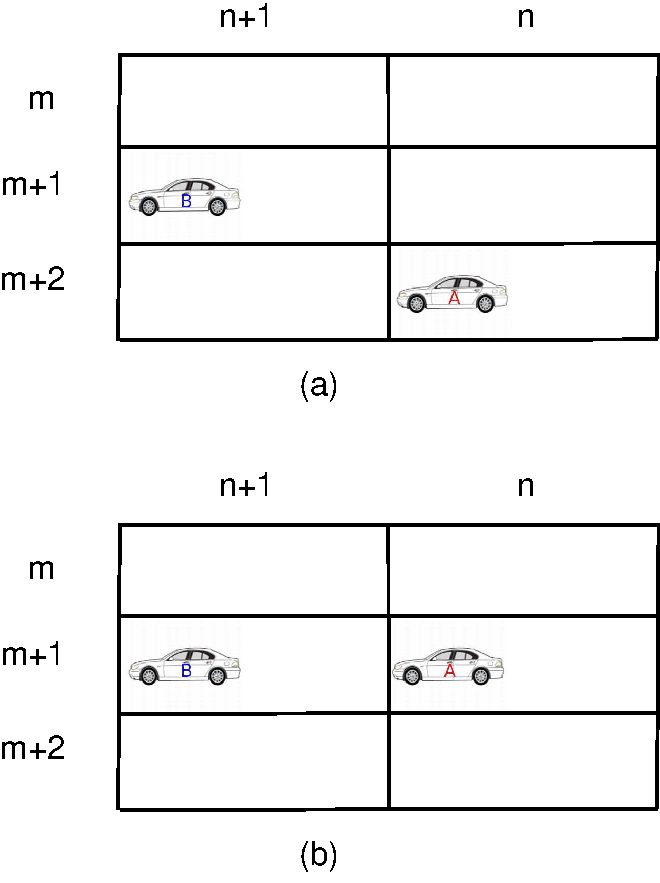
\includegraphics[width=0.5\textwidth]{diagrammi/Surpass}
\caption{Interazione tra auto nello stesso segmento}
\label{fig:surpass}
\end{center}
\end{figure}
La figura~\ref{fig:surpass} rappresenta le situazioni che si possono creare nel momento in cui un'auto percorre un segmento di pista in cui è presente un altra auto.

Individuare le auto sorpassate a seguito della mossa che un'auto (chiamiamola A) sta effettuando è semplice: detto $T_{en_X}$ il tempo di ingresso di un'auto X nel segmento e $T_{ex_X}$ il suo tempo di uscita, l'insieme delle auto $\mathcal{S}$ sorpassate da A in quel segmento sarà:
\[ \mathcal{S} = \{ X \mid T_{en_X} \leq T_{en_A} \;\wedge\; T_{ex_X} > T_{ex_A}\} \]

Nel momento in cui l'auto A effettua il suo turno sono noti:
\begin{itemize}
\item $T_{en_B}^{n+1}$: il tempo di ingresso di B nel segmento $n+1$,
\item $T_{ex_B}^{n+1}$: il tempo di uscita di B dal segmento $n+1$,
\item $L_{en_B}^{n+1}$: la corsia di ingresso di B nel segmento $n+1$,
\item $L_{ex_B}^{n+1}$: la corsia di uscita di B dal segmento $n+1$,
\item $T_{en_A}^{n+1}$: il tempo di ingresso di A nel segmento $n+1$,
\item $L_{en_A}^{n+1}$: la corsia di ingresso di A nel segmento $n+1$,
\item $L_{ex_A}^{n+1}$: la corsia di uscita di A dal segmento $n+1$ (scelta dall'auto quindi si può considerare fissata).
\end{itemize}
Obiettivo dell'algoritmo è quindi il calcolo di $T_{ex_A}^{n+1}$. Sia $T_{lc}$ il tempo che un'auto impiega a spostarsi da una corsia ad una adiacente: esso è considerato fisso ed uguale per tutte le auto e ogni auto può spostarsi di una sola corsia per ogni segmento.
Come precondizione si ha inoltre che $T_{en_B}^{n+1} \leq T_{en_A}^{n+1}$ poiché B si è spostata in quel segmento prima di A, e che $T_{en_A}^{n+1} \leq T_{ex_B}^{n+1}$ altrimenti lo \sched{} avrebbe eletto B per l'esecuzione al posto di A.

Per poter calcolare il tempo di uscita di A dal segmento $n+1$ è necessario prima valutare se B interferisce con la mossa di A.
Considerando lo scenario~(a) di figura~\ref{fig:surpass} possiamo distinguere due casi:
\begin{enumerate}
\item $L_{ex_A}^{n+1} = m+2$: non vi è alcuna interferenza da parte di B poiché la corsia $m+2$ è libera.
\item $L_{ex_A}^{n+1} = m+1$:
        \begin{enumerate}
        \item $L_{en_B}^{n+1} = m+2$: A sta seguendo esattamente la stessa traiettoria che ha seguito B per percorrere il segmento $n+1$ ed è quindi corretto che l'auto A si accodi a B e non possa superarla.
        \item $L_{en_B}^{n+1}  = m+1$: A cerca di inserirsi davanti a B tagliandole la strada; tuttavia, visto che $T_{en_B}^{n+1} \leq T_{en_A}^{n+1}$, vale anche che $T_{en_B}^{n+1} \leq T_{en_A}^{n+1} + T_{lc}$ e non è quindi possibile che A si posizioni davanti a B.
        \item $L_{en_B}^{n+1} = m$: A e B si spostano entrambe sulla stessa corsia $m+1$ provenendo da corsie differenti ma visto che $T_{en_B}^{n+1} \leq T_{en_A}^{n+1}$ allora vale anche $T_{en_B}^{n+1} + T_{lc} \leq T_{en_A}^{n+1} + T_{lc}$ e di conseguenza A può solo accodarsi a B.
        \end{enumerate}
\end{enumerate}

Per quanto riguarda lo scenario~(b) di figura~\ref{fig:surpass} vi sono due casi:
\begin{enumerate}
\item $L_{ex_A}^{n+1} = m+2$ oppure $L_{ex_A}^{n+1} = m$: non vi è alcuna interferenza da parte di B poiché le corsie sono libere.
\item $L_{ex_A}^{n+1} = m+1$:
        \begin{enumerate}
        \item $L_{en_B}^{n+1} = m+1$: A si accoda a B (vedi caso 1.a dello scenario (a)).
        \item $L_{en_B}^{n+1} = m+2$ oppure $L_{en_B}^{n+1} = m$: A cerca di inserirsi davanti a B prima che questa occupi la corsia $m+1$ e se $T_{en_B}^{n+1} + T_{lc} < T_{en_A}^{n+1}$ vuol dire che A deve accodarsi a B, altrimenti è A ed essere in testa e non viene quindi influenzata dalla presenza di B.
        \end{enumerate}
\end{enumerate}

Nei casi in cui non vi è interferenza da parte di B nella mossa di A, $T_{ex_A}^{n+1}$ viene calcolato solo sulla base delle caratteristiche dell'auto e della pista.
Nei casi in cui A deve accodarsi a B viene aggiunto il vincolo che $T_{ex_A}^{n+1} > T_{ex_B}^{n+1}$ e calcolata la velocità di uscita di conseguenza.

La procedura di sosta ai \textit{box} differisce nel calcolo del tempo di percorrenza rispetto agli altri segmenti, tuttavia si integra perfettamente nell'algoritmo citato in precedenza in quanto l'auto rimane comunque soggetta ai meccanismi di uno spostamento generico sulla pista quali il cambio corsia e il sorpasso.


L'ultima considerazione riguarda l'influenza che il fattore di \textit{simulation speed} può avere sulla competizione, ed anche in questo caso è facile convincersi che la velocità con la quale viene eseguita la simulazione non influenza in alcun modo i tempi di percorrenza delle auto. Il fattore di \textit{simulation speed} infatti viene implementato aumentando o riducendo il periodo di pausa che lo \sched{} fa trascorrere tra il rilascio della componente \track{} da parte di un processo e la concessione di tale risorsa ad un altro. Tale pausa è introdotta artificialmente per rallentare l'evolvere della simulazione e renderla quindi fruibile dall'utente.

\section{Non determinismo}
Per quanto riguarda la simulazione si ha del non determinismo nel momento in cui l'ordine di esecuzione (accesso a \track{}) non dipende solo dal tempo di prenotazione e non può essere quindi predetto.

Il non determinismo è considerato indesiderato nel momento in cui uno dei possibili ordini di esecuzione può portare ad uno stato inconsistente della simulazione.

Ricordando quanto già scritto precedentemente, l'unico caso in cui l'ordine di accesso a \track{} non dipende solo dal tempo indicato nella prenotazione presso \sched{} è in presenza di tempi di prenotazione uguali. Adottando una politica di ordinamento \textit{FIFO within priorities} si ha che l'ordine di esecuzione dei processi prenotati nel caso appena citato dipende anche dall'ordine di prenotazione, avendo essi la stessa priorità (tempo di prenotazione indicato).

Un esempio di non determinismo si ha alla partenza della gara, tuttavia, come spiegato in~\ref{sec:partenza}, tale non determinismo non influenza il risultato della simulazione e non è di conseguenza nocivo.

\begin{figure}
\begin{center}
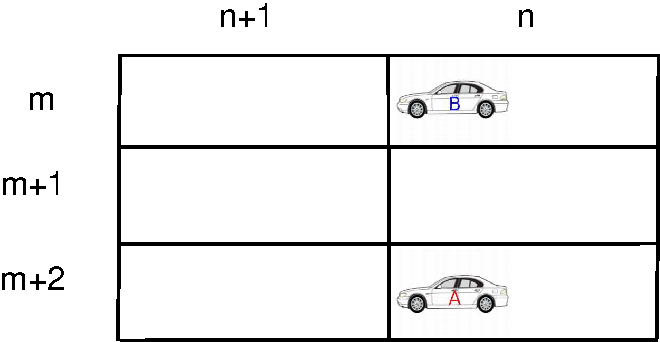
\includegraphics[width=0.6\textwidth]{diagrammi/NonDet}
\caption{Esemplificazione di una situazione di non determinismo}
\label{fig:nonDet}
\end{center}
\end{figure}

Un altro caso di non determinismo, che però influenza il risulato della simulazione, è riportato in figura~\ref{fig:nonDet} assumendo che:
\begin{itemize}
\item le auto e i piloti abbiano caratteristiche identiche;
\item $T_{en_A}^{n+1} = T_{en_B}^{n+1}$: le auto abbiano tempi di ingresso uguali;
\item $V_{en_A}^{n+1} = V_{en_B}^{n+1}$: le auto abbiano velocità di ingresso uguali.
\end{itemize}

Sotto queste ipotesi non vi sono problemi di interazione tra le auto finché $L_{ex_A}^{n+1} \neq L_{ex_B}^{n+1}$ poiché, avendo traiettorie che non si intersecano, i tempi di percorrenza dell'una non sono influenzabili in alcun modo dall'altra.

Se tuttavia si presentasse il caso in cui $L_{ex_A}^{n+1} = L_{ex_B}^{n+1}$ allora vi sarebbe del non determinismo, in quanto il tempo di percorrenza del segmento senza considerare l'influenza delle altre auto sarebbe il medesimo e, per quanto visto in~\ref{sec:percorrenza}, la prima auto ad eseguire sarà quindi anche la prima auto ad uscire dal segmento e conseguentemente la seconda auto si dovrà accodare alla prima, facendo registrare un tempo di uscita dal segmento leggermente maggiore.

In questo caso il non determinismo risulta desiderabile, infatti, anche considerando la corrsipondente situazione nella realtà, non è chiaro qualle delle auto dare la precedenza all'altra e quindi accodarsi.
Non vi sono motivi validi per preferire un pilota rispetto ad un altro quindi, piuttosto di effettuare una scelta algoritmica, si preferisce lasciare al caso la scelta.



\section{Deadlocks}
Durante la fase di progettazione del sistema abbiamo posto particolare attenzione alla prevenzione di situazioni di \textit{deadlock}.

In particolare ci siamo resi conto che il flusso di notifiche presente nel sistema poteva essere fonte di situazioni di stallo.
In primo luogo vale la pena notare che, grazie alla struttura interna di \evdisp{} descritta in~\ref{sec:dispatcherImpl}, non è possibile che si creino \textit{deadlocks} coinvolgenti tale componente.

Questo fatto deriva direttamente dall'uso di chiamate non bloccanti tra \textit{front-end} e \textit{back-end} che impedisce strutturalmente il concretizzarsi della situazione di attesa circolare necessaria alla formazione di \textit{deadlocks}.

Questa soluzione ci assicura l'assenza di stallo causato dalle notifiche, poiché la propagazione di queste ultime coinvolge \evdisp{} che, come appena spiegato, previene sistematicamente la formazione di \textit{deadlock}.

Un'altra situazione pericolosa da questo punto di vista è stata individuata in fase di progettazione nella comunicazione tra le componenti \track{}, \team{} e \car{} durante la sosta per il rifornimento. Questo problema viene ampiamente trattato e risolto come descritto in~\ref{sec:rifornimento}.

Eliminata quindi la possibilità di \textit{deadlocks} comprendenti \evdisp{} e appurato che la comunicazione tra \track{}, \team{} e \car{} è libera da stallo, si può affermare che nel sistema non possono verificarsi situazioni di \textit{deadlock} poiché, per quanto riguarda le rimanenti comunicazioni, non sussiste la precondizione di attesa circolare tra le componenti.
\section{Realismo}
\subsection*{Fisico}
Al fine di ottenere un buon livello di realismo della simulazione da un punto di vista fisico, abbiamo deciso di far dipendere le \textit{performance} dell'auto da diversi fattori modellando i fenomeni fisici coinvolti nel miglior modo possibile, con particolare attenzione alla decelerazione.

Nella seguente tabella vengono riportati i valori utilizzati nel modello fisico della simulazione e da quali parametri di configurazione tali valori dipendono.

\begin{center}
\begin{tabular}{|l|l|}
\hline
\textbf{Valore} & \textbf{Ricavato da} \\
\hline
\multirow{5}{*}{Velocità massima in curva} & Raggio di curvatura\\
& Inclinazione del tratto\\
& Condizioni atmosferiche\\
& Tipo di pneumatici\\
& Usura dei pneumatici\\
\hline
\multirow{8}{*}{Accelerazione/Decelerazione massima} & Potenza del motore/dei freni\\
& Peso dell'auto\\
& Peso del carburante\\
& Peso del pilota\\
& Inclinazione del tratto\\
& Condizioni atmosferiche\\
& Tipo di pneumatici\\
& Usura dei pneumatici\\
\hline
\multirow{3}{*}{Consumo dei pneumatici} & Raggio di curvatura\\
& Tipo di pneumatici\\
& Condizioni atmosferiche\\
\hline
Consumo di carburante & Inclinazione del tratto\\
\hline
\end{tabular}
\end{center}

Considerando la fase di decelerazione che un'auto deve generalmente intraprendere prima di entrare in curva o prima di accedere alla \textit{pit lane}, è stato necessario introdurre nelle meccaniche di simulazione il calcolo della tabella di preelaborazione. Questo principalmente per evitare che le auto arrivassero all'entrata della curva e, non avendo il tempo di frenare, uscissero di pista sistematicamente.

\subsection*{Dinamiche di gara}
Per quanto riguarda il realismo nelle dinamiche di gara, abbiamo considerato la possibilità per un'auto di ritirarsi dalla competizione a seguito di:
\begin{itemize}
\item uscita di pista per velocità troppo elevata;
\item uscita di pista per evitare incidenti qualora l'auto non riesca a frenare in tempo per evitare gli altri concorrenti;
\item esplosione pneumatici a causa di eccessiva usura;
\item esaurimento del carburante;
\item potenza del motore insufficiente a percorrere il tratto.
\end{itemize}

Si è cercato poi di descrivere l'interazione tra le auto in uno stesso segmento in modo preciso, per poter distinguere le condizioni di sorpasso e quelle di accodamento anche in base alla traiettoria di un'auto. Limitare il cambio di corsia ad uno solo per segmento è stato utile per avere un maggior controllo sull'algoritmo di percorrenza di un segmento e sull'aderenza della simulazione alla realtà.
